
% 2018 KTS
% Dancing links package

\documentclass[xcolor=svgnames]{beamer}

\usetheme[titleformat=smallcaps,subsectionpage=progressbar]{metropolis}
\metroset{outer/progressbar=head}

\usepackage{fancyvrb}
\usepackage{kotex}

\setsanshangulfont{Kakao OTF}[
  Script=Hangul,
  Language=Korean,
  BoldFont=* Bold,
  InterLatinCJK=.125em,
]

\usepackage{dlx}


% title
\title{댄싱 링크 패키지}
\subtitle{텍으로 퍼즐 조판하기}
\date{2018년 2월 3일}
\author{남수진}
\institute{
  2018 한국텍학회 학술대회 및 정기총회 \\
  판교 스타트업캠퍼스 1동 2층, 세미나실 1}
\titlegraphic{\hfill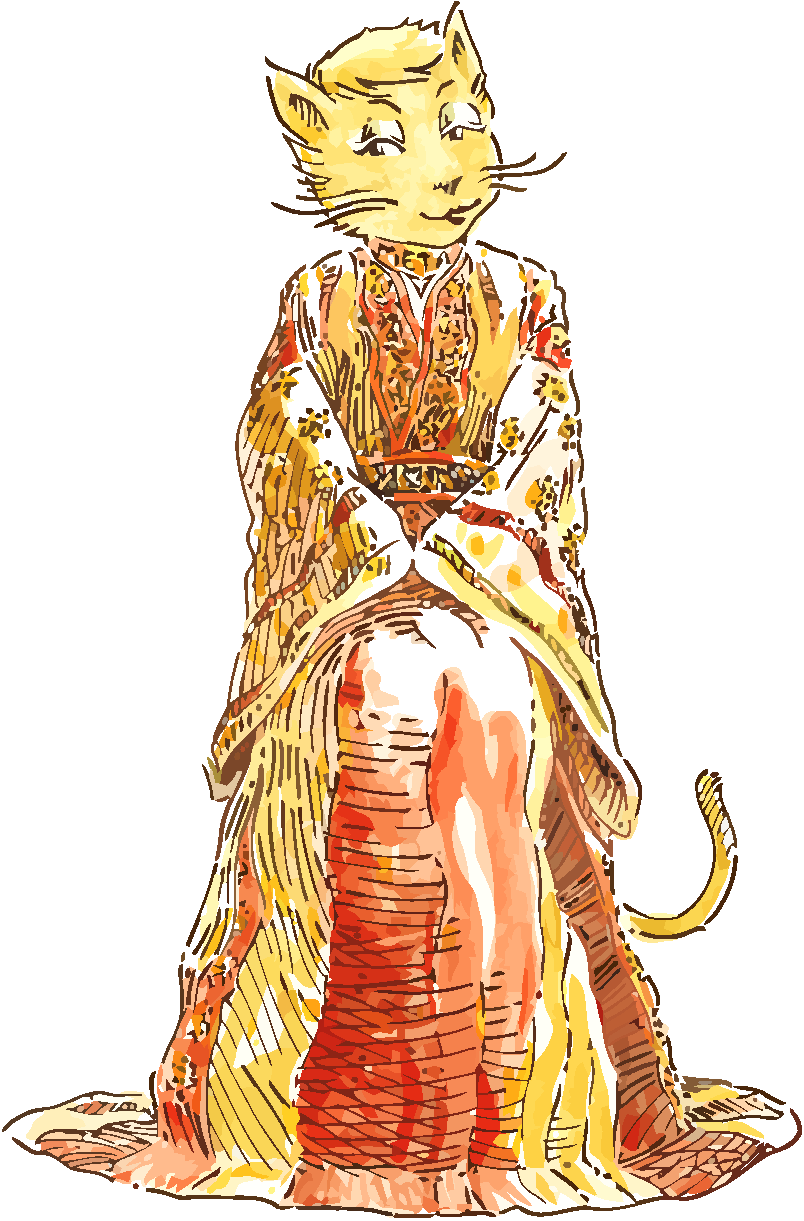
\includegraphics[height=30mm]{imgs/meta.pdf}}


%%
\begin{document}

\maketitle

%
\begin{frame}{목차}
  \setbeamertemplate{section in toc}[sections numbered]
  \tableofcontents
\end{frame}


%%
\section{댄싱 링크, Dancing links}

\let\a\alert
\def\g{\color{LightGray}}

%
\begin{frame}{Exact cover 문제}
  다음 행렬에서, 모든 열을 1로 만드는 행들을 찾아라.
  {\Large\boldmath
    $$
    \bordermatrix{
      \mathstrut&&&&&&&\cr
      &0&0&1&0&1&1&0\cr
      &1&0&0&1&0&0&1\cr
      &0&1&1&0&0&1&0\cr
      &1&0&0&1&0&0&0\cr
      &0&1&0&0&0&0&1\cr
      &0&0&0&1&1&0&1}
    $$}
\end{frame}

%
\begin{frame}{Exact cover 문제}
  다음 행렬에서, 모든 열을 1로 만드는 행들을 찾아라.
  {\Large\boldmath
    $$
    \bordermatrix{
      \mathstrut&&&&&&&\cr  
      &0&0&1&0&1&1&0\cr
      &\g1&\g0&\g0&\g1&\g0&\g0&\g1\cr
      &\g0&\g1&\g1&\g0&\g0&\g1&\g0\cr
      &1&0&0&1&0&0&0\cr
      &0&1&0&0&0&0&1\cr
      &\g0&\g0&\g0&\g1&\g1&\g0&\g1}
    $$}
\end{frame}

%
\begin{frame}{Exact cover 문제}
\Large\boldmath
  \begin{figure}[!htb]
    \hskip-17mm\begin{minipage}{.7\textwidth}
      \centering
      $\bordermatrix{
  \strut&&&&&&&\cr
  &0&0&1&0&1&1&0\cr
  &1&0&0&1&0&0&1\cr
  &0&1&1&0&0&1&0\cr
  &1&0&0&1&0&0&0\cr
  &0&1&0&0&0&0&1\cr
  &0&0&0&1&1&0&1}\ \Rightarrow$
    \end{minipage}%
    \begin{minipage}{.3\textwidth}
      \centering
  $
  \begin{array}{ccccccc}
    A & B & C & D & E & F & G\\
    C & E & F &&&&\\
    A & D & G &&&&\\
    B & C & F &&&&\\
    A & D &&&&&\\
    B & G &&&&&\\
    D & E & G &&&&
  \end{array}
  $
    \end{minipage}
\end{figure}
\end{frame}

\renewcommand\arraystretch{1.2}

\begin{frame}{알고리즘 엑스}
\Large\boldmath
  $$
  \begin{array}{ccccccc}
    A & B & C & D & E & F & G\\
    C & E & F &&&&\\
    A & D & G &&&&\\
    B & C & F &&&&\\
    A & D &&&&&\\
    B & G &&&&&\\
    D & E & G &&&&
  \end{array}
  $$
\end{frame}

%
\begin{frame}{알고리즘 엑스, 비결정적}
\Large\boldmath
  $$
  \begin{array}{ccccccc}
    \a A & B & C & \a D & E & F & \a G\\
    C & E & F &&&&\\
    \a A & \a D & \a G &&&&\\
    B & C & F &&&&\\
    A & D &&&&&\\
    B & G &&&&&\\
    D & E & G &&&&
  \end{array}
  $$
\end{frame}

%
\begin{frame}{알고리즘 엑스, 재귀적}
\Large\boldmath
  $$
  \begin{array}{ccccccc}
    \a A & B & C & \a D & E & F & \a G\\
    C & E & F &&&&\\
    \a A & \a D & \a G &&&&\\
    B & C & F &&&&\\
    \g A & \g D &&&&&\\
    \g B & \g G &&&&&\\
    \g D & \g E & \g G &&&&
  \end{array}
  $$
\end{frame}

%
\begin{frame}{알고리즘 엑스}
\Large\boldmath
  $$
  \begin{array}{ccccccc}
    \a A & B & \a C & \a D & \a E & \a F & \a G\\
    \a C & \a E & \a F &&&&\\
    \a A & \a D & \a G &&&&\\
    B & C & F &&&&\\
    \g A & \g D &&&&&\\
    \g B & \g G &&&&&\\
    \g D & \g E & \g G &&&&
  \end{array}
  $$
\end{frame}

%
\begin{frame}{알고리즘 엑스, 깊이 우선 탐색}
  \Large\boldmath
  $$
  \begin{array}{ccccccc}
    \a A & B & \a C & \a D & \a E & \a F & \a G\\
    \a C & \a E & \a F &&&&\\
    \a A & \a D & \a G &&&&\\
    \g B & \g C & \g F &&&&\\
    \g A & \g D &&&&&\\
    \g B & \g G &&&&&\\
    \g D & \g E & \g G &&&&
  \end{array}
  $$
\end{frame}

%
\begin{frame}{알고리즘 엑스, 백트래킹}
\Large\boldmath
  $$
  \begin{array}{ccccccc}
    A & B & C & D & E & F & G\\
    C & E & F &&&&\\
    A & D & G &&&&\\
    B & C & F &&&&\\
    A & D &&&&&\\
    B & G &&&&&\\
    D & E & G &&&&
  \end{array}
  $$
\end{frame}

%
\begin{frame}{알고리즘 엑스}
\Large\boldmath
  $$
  \begin{array}{ccccccc}
    \a A & B & C & \a D & E & F & G\\
    C & E & F &&&&\\
    A & D & G &&&&\\
    B & C & F &&&&\\
    \a A & \a D &&&&&\\
    B & G &&&&&\\
    D & E & G &&&&
  \end{array}
  $$
\end{frame}

%
\begin{frame}{알고리즘 엑스}
\Large\boldmath
  $$
  \begin{array}{ccccccc}
    \a A & B & C & \a D & E & F & G\\
    C & E & F &&&&\\
    \g A & \g D & \g G &&&&\\
    B & C & F &&&&\\
    \a A & \a D &&&&&\\
    B & G &&&&&\\
    \g D & \g E & \g G &&&&
  \end{array}
  $$
\end{frame}

%
\begin{frame}{알고리즘 엑스}
\Large\boldmath
  $$
  \begin{array}{ccccccc}
    \a A & B & \a C & \a D & \a E & \a F & G\\
    \a C & \a E & \a F &&&&\\
    \g A & \g D & \g G &&&&\\
    B & C & F &&&&\\
    \a A & \a D &&&&&\\
    B & G &&&&&\\
    \g D & \g E & \g G &&&&
  \end{array}
  $$
\end{frame}

%
\begin{frame}{알고리즘 엑스}
\Large\boldmath
  $$
  \begin{array}{ccccccc}
    \a A & B & \a C & \a D & \a E & \a F & G\\
    \a C & \a E & \a F &&&&\\
    \g A & \g D & \g G &&&&\\
    \g B & \g C & \g F &&&&\\
    \a A & \a D &&&&&\\
    B & G &&&&&\\
    \g D & \g E & \g G &&&&
  \end{array}
  $$
\end{frame}

%
\begin{frame}{알고리즘 엑스}
\Large\boldmath
$$
  \begin{array}{ccccccc}
    \a A & \a B & \a C & \a D & \a E & \a F & \a G\\
    \a C & \a E & \a F &&&&\\
    \g A & \g D & \g G &&&&\\
    \g B & \g C & \g F &&&&\\
    \a A & \a D &&&&&\\
    \a B & \a G &&&&&\\
    \g D & \g E & \g G &&&&
  \end{array}
  $$
\end{frame}

%
\begin{frame}{알고리즘 엑스}
\Large\boldmath
  $$
  \begin{array}{ccccccc}
    A & B & C & D & E & F & G\\
    C & E & F &&&&\\
    A & D & G &&&&\\
    B & C & F &&&&\\
    A & D &&&&&\\
    B & G &&&&&\\
    D & E & G &&&&
  \end{array}
  $$
\end{frame}

%
\begin{frame}{댄싱 링크}
  \begin{itemize}
  \item 비결정적, 재귀적, 깊이 우선 탐색, 백트래킹
  \item 알고리즘 엑스를 효율적으로 구현하는 하나의 기법
  \item \href{https://www.youtube.com/watch?v=pN76VICZiKU&start=100}
    {알고리즘이 진행되면서 변화하는 링크의 모양이 춤을 연상 시킴}
  \end{itemize}
  \vspace{-3mm}
  \begin{center}
    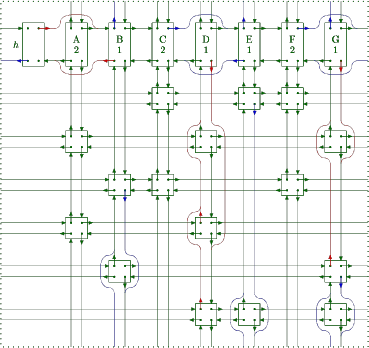
\includegraphics[height=60mm]{imgs/cdance-4.png}
  \end{center}
\end{frame}


%%
\section{펜토미노 타일링}

%
\begin{frame}{펜토미노}
  \begin{center}
  {\Large 12 조각} \\
  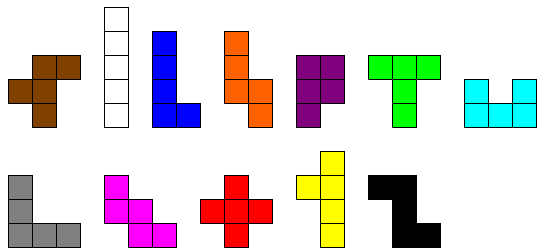
\includegraphics[height=4.5cm]{imgs/pentominoes.png}
  \end{center}
\end{frame}

%
\begin{frame}[fragile]{펜토미노 타일링}
\begin{verbatim}
\usepackage{dlx}
\pentomino{5mm}{6}{10}{1}.
\end{verbatim}
\vspace{-5mm}
\pentomino{5mm}{6}{10}{1}.
\vspace{-5mm}
\begin{verbatim}
\pentomino{5mm}{3}{20}{1}.
\end{verbatim}
\vspace{-5mm}
\pentomino{5mm}{3}{20}{1}.
\end{frame}

%
\begin{frame}[fragile]{펜토미노 타일링}
\begin{verbatim}
\pentomino{5mm}{5}{12}{1}.
\end{verbatim}
\vspace{-5mm}
\pentomino{5mm}{5}{12}{1}.
\vspace{-5mm}
\begin{verbatim}
\pentomino{5mm}{4}{15}{1}.
\end{verbatim}
\vspace{-5mm}
\pentomino{5mm}{4}{15}{1}.
\end{frame}


%%
\section{수도쿠}

%
\begin{frame}[fragile]{수도쿠}
  \begin{Verbatim}[fontsize=\small]
\usepackage{dlx}
\Sudoku{9.......6.3.4....9...915.8..8.5..7..%
..3.9.4....2..1.9.32176....6..1.2.3.8...5...1}
\end{Verbatim}  
\begin{center}
  \Sudoku{9.......6.3.4....9...915.8..8.5..7..%
    ..3.9.4....2..1.9.32176....6..1.2.3.8...5...1}
\end{center}
\end{frame}

%
\begin{frame}[fragile]{수도쿠}
\begin{Verbatim}[fontsize=\small]
\usepackage{dlx}
\Sudoku*{9.......6.3.4....9...915.8..8.5..7..%
..3.9.4....2..1.9.32176....6..1.2.3.8...5...1}
\end{Verbatim}
\begin{center}
  \Sudoku*{9.......6.3.4....9...915.8..8.5..7..%
    ..3.9.4....2..1.9.32176....6..1.2.3.8...5...1}
\end{center}
\end{frame}


%%
\section{여왕 배치 문제}

%
\begin{frame}[fragile]{여왕 배치 문제}
\begin{verbatim}
\usepackage{dlx}
\queens{4}.
\end{verbatim}
\vspace{-10mm}
\queens{4}.
\end{frame}

%
\begin{frame}[fragile]{여왕 배치 문제}
\begin{verbatim}
\usepackage{dlx}
\queens{8}{2}.
\end{verbatim}
\vspace{-10mm}
\queens{8}{2}.
\end{frame}


%
\begin{frame}{참고}
  \begin{itemize}
  \item \href{http://www-cs-faculty.stanford.edu/~knuth/fasc5c.ps.gz}
    {\textsc{The Art of Computer Programming Pre-Fascicle 5c}}
  \item \href{https://github.com/sjnam/lua-dancing-links}
    {lua-dancing-links}
  \end{itemize}
\end{frame}

%
\begin{frame}[standout]
  감사합니다
\end{frame}

\end{document}

